\documentclass[a4paper,12pt,landscape,twocolumn]{article}

\usepackage{préambule}
\usetikzlibrary{calc,arrows.meta}
\usepackage{clipboard}

\geometry{left=1cm}
\setlength{\columnsep}{0.8cm}

\newcommand{\myarrow}{{Latex[length=1mm, width=1.5mm]}-{Latex[length=1mm, width=1.5mm]}}

\TitreDEvaluation{Évaluation calcul littéral}
\author{}
\date{15 avril}

\begin{document}

\renewcommand{\arraystretch}{1.4}

\Copy{Contenu}{
	\maketitle

	\begin{exercice}\

		\begin{center}
			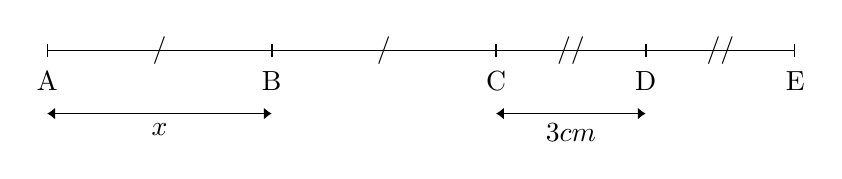
\begin{tikzpicture}[scale=0.95]
				\coordinate (A) at (0,0);
				\coordinate (B) at (3,0);
				\coordinate (C) at (6,0);
				\coordinate (D) at (8,0);
				\coordinate (E) at (10,0);
				\draw[|-|] (A) -- node {/} (B);
				\draw[|-|] (B) -- node {/} (C);
				\draw[|-|] (C) -- node {//} (D);
				\draw[|-|] (D) -- node {//} (E);

				\foreach \p in {A,B,C,D,E} {
						\node[below] at ($(\p) - (0,0.15)$) {\p};
					}

				\draw[\myarrow] ($(A) - (0,0.84)$) -- node[below] {$x$} ($(B) - (0,0.84)$);
				\draw[\myarrow] ($(C) - (0,0.84)$) -- node[below] {$3cm$} ($(D) - (0,0.84)$);
			\end{tikzpicture}
		\end{center}

		On appelle $x$ la distance AB. De plus, on sait que la distance CD est 3cm.

		Écrire une expression représentant la distance AE : \dotfill

		\vspace{1em}

		\begin{center}
			\begin{tikzpicture}[scale=0.95]
				\coordinate (A) at (0,0);
				\coordinate (B) at (2.5,0);
				\coordinate (E) at (5,0);
				\coordinate (D) at (7.5,0);
				\coordinate (C) at (10,0);
				\draw[|-|] (A) -- node {//} (B);
				\draw[|-|] (B) -- node {//} (E);
				\draw[|-|] (E) -- node {//} (D);
				\draw[|-|] (D) -- node {//} (C);

				\foreach \p in {A,B,C} {
						\node[below] at ($(\p) - (0,0.2)$) {\p};
					}

				\draw[\myarrow] ($(A) - (0,0.82)$) -- node[below] {$x$} ($(C) - (0,0.82)$);
			\end{tikzpicture}
		\end{center}

		On appelle $x$ la distance AC.

		Écrire une expression représentant la distance AB : \dotfill
	\end{exercice}

	\begin{exercice}\

		Calculer la valeur de l'expression $4x + 3$ pour : \vspace{0.5em}

		\begin{tabular}{llm{4cm}}
			a. & $x = 10$ & \dotfill \\ % 43
			b. & $x = 5$  & \dotfill \\ % 23
		\end{tabular}
	\end{exercice}

	\begin{exercice}\

		Calculer la valeur de l'expression $5x + 6 - 3y$ pour : \vspace{0.5em}

		\begin{tabular}{llm{4cm}}
			a. & $x = 6$ et $y = 5$   & \dotfill \\ % 21
			b. & $x = 12$ et $y = 10$ & \dotfill \\ % 36
		\end{tabular}
	\end{exercice}

	\begin{exercice}\

		Simplifier les expressions suivantes : \vspace{0.5em}
		\begin{enumerate}[label=\alph*.]
			\setlength\itemsep{5pt}
			\item $3 × x + 2 = $ \dotfill
			\item $x + x + 1{,}5 + 2{,}5 = $ \dotfill
			\item $4 × x + 1 × y  - 2 × x = $ \dotfill
		\end{enumerate}
	\end{exercice}
}

\newpage

\setcounter{exercice}{0}
\Paste{Contenu}

\end{document}